In this paper we shall explore sequences of billiard ball collisions. In particular, we look at the 

\section{Setup}

We will imagine an infinitesimally small billiard ball on a square table. The ball will start at some initial position inside of the table and with some velocity. We will assume that the ball is massless and frictionless, and that there is no gravity.

We will assume ideal, elastic collisions so that the ball conserves both kinetic energy and momentum when it hits a wall. To be more precise, when the ball collides with an edge of the table, the ball's velocity will be reflected across the line perpendicular to the edge of the table at the point of collision. In other words, the angle of the incoming velocity will be the same as the outgoing velocity. Figure \ref{fig:collision-angle} shows the general mechanics of a collision.

\begin{figure}
  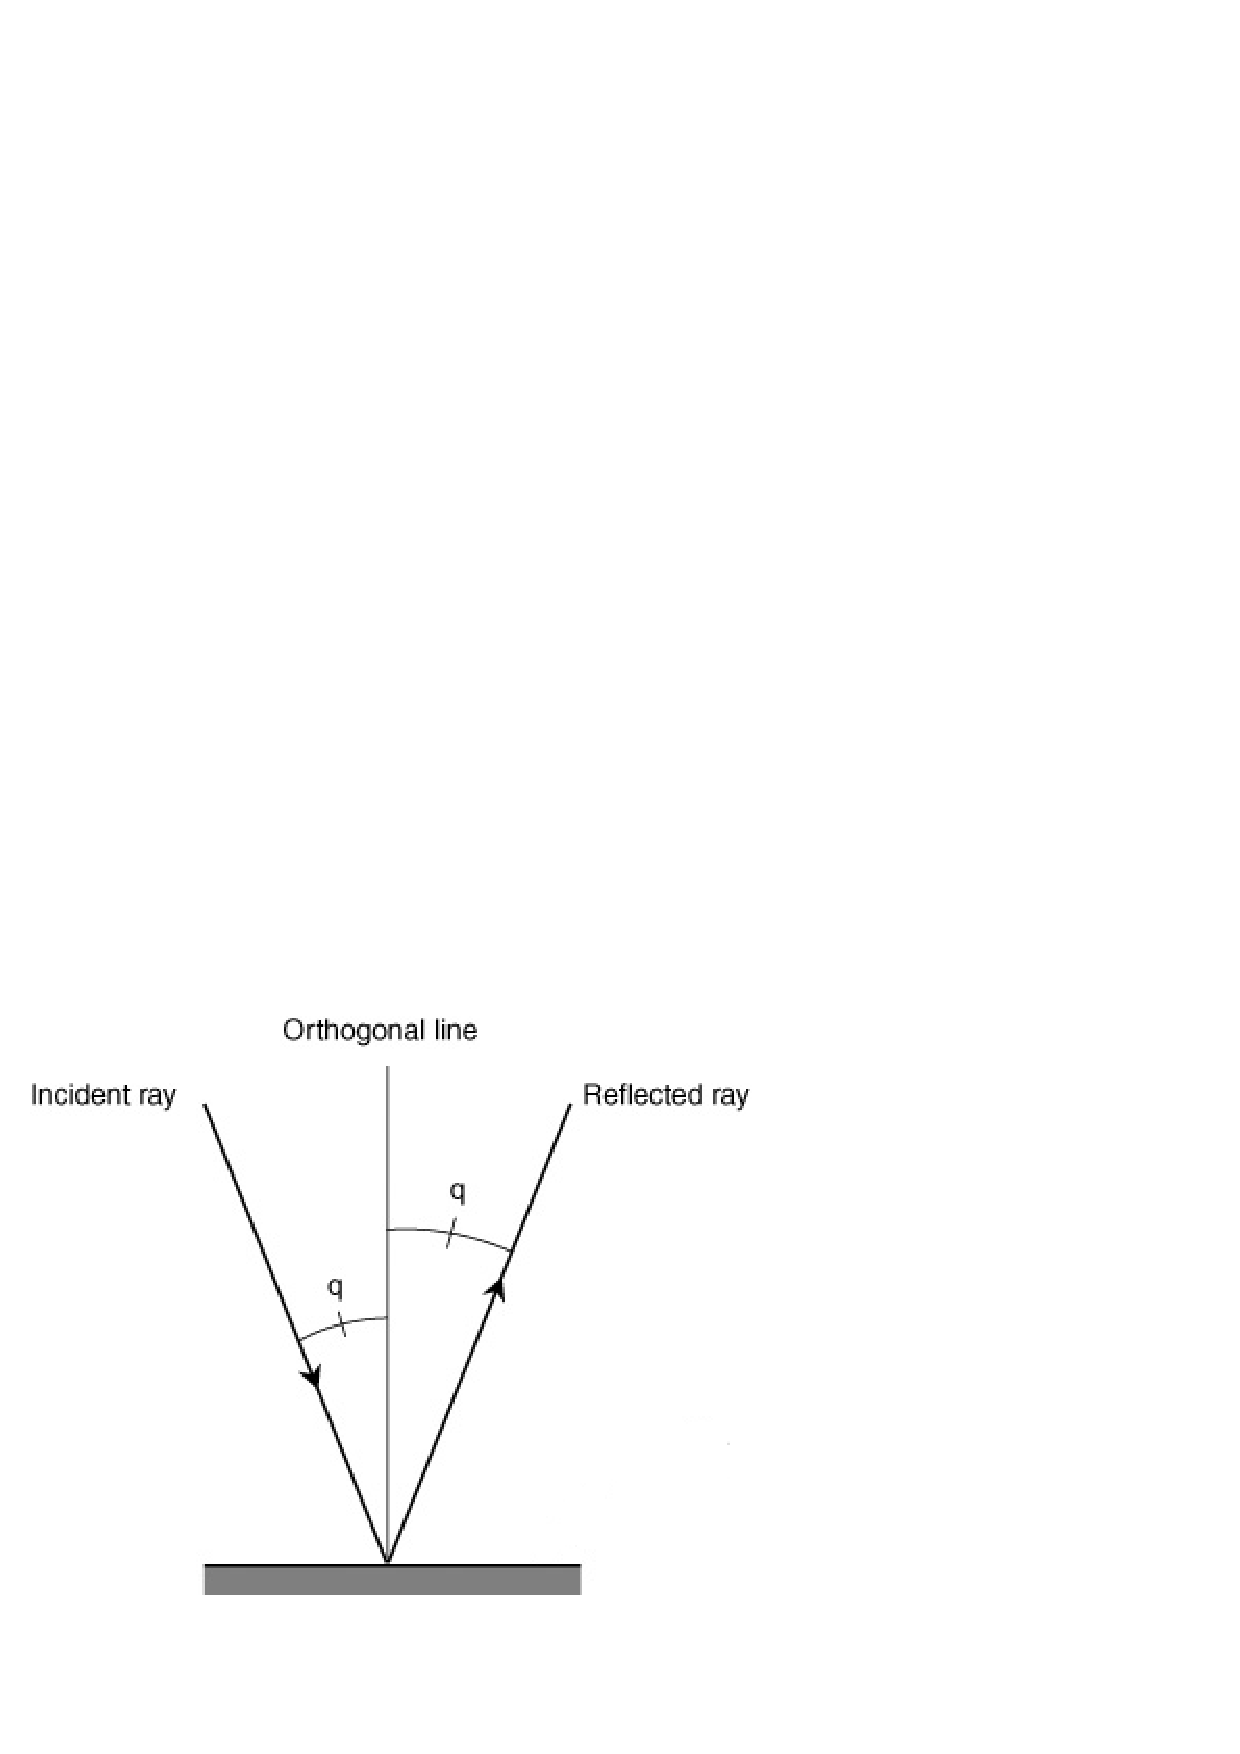
\includegraphics[width=2in]{particle_collision.png}
  \caption{\label{fig:collision-angle}Mechanics of a Billiards Ball Colliding with a Table Edge}
\end{figure}
